%	This is written by Zhiyang Ong as a template for writing reports.

%	The MIT License (MIT)

%	Copyright (c) <2014> <Zhiyang Ong>

%	Permission is hereby granted, free of charge, to any person obtaining a copy of this software and associated documentation files (the "Software"), to deal in the Software without restriction, including without limitation the rights to use, copy, modify, merge, publish, distribute, sublicense, and/or sell copies of the Software, and to permit persons to whom the Software is furnished to do so, subject to the following conditions:

%	The above copyright notice and this permission notice shall be included in all copies or substantial portions of the Software.

%	THE SOFTWARE IS PROVIDED "AS IS", WITHOUT WARRANTY OF ANY KIND, EXPRESS OR IMPLIED, INCLUDING BUT NOT LIMITED TO THE WARRANTIES OF MERCHANTABILITY, FITNESS FOR A PARTICULAR PURPOSE AND NONINFRINGEMENT. IN NO EVENT SHALL THE AUTHORS OR COPYRIGHT HOLDERS BE LIABLE FOR ANY CLAIM, DAMAGES OR OTHER LIABILITY, WHETHER IN AN ACTION OF CONTRACT, TORT OR OTHERWISE, ARISING FROM, OUT OF OR IN CONNECTION WITH THE SOFTWARE OR THE USE OR OTHER DEALINGS IN THE SOFTWARE.

%	Email address: echo "cukj -wb- 23wU4X5M589 TROJANS cqkH wiuz2y 0f Mw Stanford" | awk '{ sub("23wU4X5M589","F.d_c_b. ") sub("Stanford","d0mA1n"); print $5, $2, $8; for (i=1; i<=1; i++) print "6\b"; print $9, $7, $6 }' | sed y/kqcbuHwM62z/gnotrzadqmC/ | tr 'q' ' ' | tr -d [:cntrl:] | tr -d 'ir' | tr y "\n"

%%%%%%%%%%%%%%%%%%%%%%%%%%%%%%%%%%%%%%%%%%%%%%









%%%%%%%%%%%%%%%%%%%%%%%%%%%%%%%%%%%%%%%%%%%%%%
%	Preamble.
\documentclass[letterpaper,12pt]{report}
%%%%%%%%%%%%%%%%%%%%%%%%%%%%%%%%%%%%%%%%%%%%%
%
%	Importing LaTeX source files, without quoting the ".tex" extension.
%
%%%%%%%%%%%%%%%%%%%%%%%%%%%%%%%%%%%%%%%%%%%%%

%%%%%%%%%%%%%%%%%%%%%%%%%%%%%%%%%%%%%%%%%%%%%
%	File containing the LaTeX preamble.
\input{./others/preamble}
%	Enable the use of right-sided cases.
\usepackage{mathtools}
%\usepackage{extarrows}






%%%%%%%%%%%%%%%%%%%%%%%%%%%%%%%%%%%%%%%%%%%%%
%
%	Start of LaTeX document
%
%%%%%%%%%%%%%%%%%%%%%%%%%%%%%%%%%%%%%%%%%%%%%
\begin{document}

%%%%%%%%%%%%%%%%%%%%%%%%%%%%%%%%%%%%%%%%%
%	File containing a list of ``the 68 predefined internal colors of the {\tt dvips} PostScript driver'' \cite{Kopka04} 
%	This allows me to use any of these ``68 predefined internal colors''
\input{./others/list_of_colors.def}









%%%%%%%%%%%%%%%%%%%%%%%%%%%%%%%%%%%%%%%%%%%%%
%%%%%%%%%%%%%%%%%%%%%%%%%%%%%%%%%%%%%%%%%%%%%
%
%	Information for Top Matter / Title page
%
%%%%%%%%%%%%%%%%%%%%%%%%%%%%%%%%%%%%%%%%%%%%%
%%%%%%%%%%%%%%%%%%%%%%%%%%%%%%%%%%%%%%%%%%%%%
%	Beginning of FRONT MATTER: title page, table of contents and prefaces
%	Note that the \vspace{length} command does NOT work for the front matter
%\frontmatter
\title{\Huge \bf Title of the Report: Some Details about the Report}

%	Indicate the date of the report.
\date{\today}

\author{{\LARGE Nome Cognome}
\thanks{Email correspondence to: \href{mailto:email-id@domain.url}{\Email\ email-id@domain.url}}
\ \\
\vspace{-4.0in}
\ \\
\ \\
\ \\
{\bf \LARGE
	Name of Organization
	\vspace{0.1cm}} \\
\hline
\ \\
{\Large \sc Name of Group/Division} \\
\ \\
\ \\
\ \\
\ \\
\ \\
\vspace{2.0in}
\ \\
{\large \sc What is this report for?} \\
{\large It is for \dots} \\
{\large and BLAH \dots}
}

%	Create the title page.
\maketitle


%%%%%%%%%%%%%%%%%%%%%%%%%%%%%%%%%%%%%%%%%%%%%
%
%	Abstract

\begin{abstract} 
Insert abstract here. \\

More stuff to be included.
\end{abstract}

%%%%%%%%%%%%%%%%%%%%%%%%%%%%%%%%%%%%%%%%%%%%%
%%%%%%%%%%%%%%%%%%%%%%%%%%%%%%%%%%%%%%%%%%%%%

% Set the page numbering to lowercase Roman numerals
\pagenumbering{roman}
% Set the initial page number of the pages in the content section to be ``i''
\setcounter{page}{1}

%%%%%%%%%%%%%%%%%%%%%%%%%%%%%%%%%%%%%%%%%
%	Revision History
%	This is written by Zhiyang Ong to record significant changes made to the report.

%	The MIT License (MIT)

%	Copyright (c) <2014> <Zhiyang Ong>

%	Permission is hereby granted, free of charge, to any person obtaining a copy of this software and associated documentation files (the "Software"), to deal in the Software without restriction, including without limitation the rights to use, copy, modify, merge, publish, distribute, sublicense, and/or sell copies of the Software, and to permit persons to whom the Software is furnished to do so, subject to the following conditions:

%	The above copyright notice and this permission notice shall be included in all copies or substantial portions of the Software.

%	THE SOFTWARE IS PROVIDED "AS IS", WITHOUT WARRANTY OF ANY KIND, EXPRESS OR IMPLIED, INCLUDING BUT NOT LIMITED TO THE WARRANTIES OF MERCHANTABILITY, FITNESS FOR A PARTICULAR PURPOSE AND NONINFRINGEMENT. IN NO EVENT SHALL THE AUTHORS OR COPYRIGHT HOLDERS BE LIABLE FOR ANY CLAIM, DAMAGES OR OTHER LIABILITY, WHETHER IN AN ACTION OF CONTRACT, TORT OR OTHERWISE, ARISING FROM, OUT OF OR IN CONNECTION WITH THE SOFTWARE OR THE USE OR OTHER DEALINGS IN THE SOFTWARE.

%	Email address: echo "cukj -wb- 23wU4X5M589 TROJANS cqkH wiuz2y 0f Mw Stanford" | awk '{ sub("23wU4X5M589","F.d_c_b. ") sub("Stanford","d0mA1n"); print $5, $2, $8; for (i=1; i<=1; i++) print "6\b"; print $9, $7, $6 }' | sed y/kqcbuHwM62z/gnotrzadqmC/ | tr 'q' ' ' | tr -d [:cntrl:] | tr -d 'ir' | tr y "\n"

%%%%%%%%%%%%%%%%%%%%%%%%%%%%%%%%%%%%%%%%%%%%%
\chapter*{Revision History}
\addcontentsline{toc}{chapter}{Revision History}
\label{chp:revisionhistory}


Revision History: \vspace{-0.3cm}
\begin{enumerate} \itemsep -4pt
\item Version 0.1, June 1, 2014. Initial copy of the report.
\item Version 0.2, June 4, 2014. Added chapter on typesetting algorithms.
\item Version 0.3, June 4, 2014. Added chapter on typesetting text, inserting figures and tables, added a subdirectory for pictures of the report, and begun a section on typesetting mathematical symbols, expressions, and equations.
\item Version 0.4, June 4, 2014. Added introductory paragraph on typesetting in \LaTeX, and referencing and citations.
\item Version 0.5, June 5, 2014. Completed section on using color in \LaTeX. In addition, I have completed another section on symbols representing \LaTeX\ and related computer languages/technologies/concepts.
\item Version 0.6, June 5, 2014. Completed chapter on typesetting (macros) in \LaTeX.
\item Version 0.7, June 8, 2014. Completed \LaTeX\ template for reports.
\end{enumerate}








%%%%%%%%%%%%%%%%%%%%%%%%%%%%%%%%%%%%%%%%%
%	Create the table of contents
\tableofcontents
%	Start the numbering of chapters from 1, instead of 0.
%\setcounter{chapter}{1}
%	Increase the depth of each section in the Table of Contents to 4.
\setcounter{secnumdepth}{4}

%	List of Figures		=> Insert Here!!!
%	List of Tables			=> Insert Here!!!
%	List of To-Do Tasks	=> Insert Here!!!
%\listoftodos





%%%%%%%%%%%%%%%%%%%%%%%%%%%%%%%%%%%%%%%%%%%%%
%%%%%%%%%%%%%%%%%%%%%%%%%%%%%%%%%%%%%%%%%%%%%
\newpage
%\mainmatter

%	Body, or main section, of the document
%	Set the page numbering to normal (Arabic) numerals
\pagenumbering{arabic}
% Set the page numbers for the body of the document
\setcounter{page}{1}





%%%%%%%%%%%%%%%%%%%%%%%%%%%%%%%%%%%%%%%%%
%	Typesetting Text in LaTeX
%	This is written by Zhiyang Ong as a template for typesetting in LaTeX.

%	The MIT License (MIT)

%	Copyright (c) <2014> <Zhiyang Ong>

%	Permission is hereby granted, free of charge, to any person obtaining a copy of this software and associated documentation files (the "Software"), to deal in the Software without restriction, including without limitation the rights to use, copy, modify, merge, publish, distribute, sublicense, and/or sell copies of the Software, and to permit persons to whom the Software is furnished to do so, subject to the following conditions:

%	The above copyright notice and this permission notice shall be included in all copies or substantial portions of the Software.

%	THE SOFTWARE IS PROVIDED "AS IS", WITHOUT WARRANTY OF ANY KIND, EXPRESS OR IMPLIED, INCLUDING BUT NOT LIMITED TO THE WARRANTIES OF MERCHANTABILITY, FITNESS FOR A PARTICULAR PURPOSE AND NONINFRINGEMENT. IN NO EVENT SHALL THE AUTHORS OR COPYRIGHT HOLDERS BE LIABLE FOR ANY CLAIM, DAMAGES OR OTHER LIABILITY, WHETHER IN AN ACTION OF CONTRACT, TORT OR OTHERWISE, ARISING FROM, OUT OF OR IN CONNECTION WITH THE SOFTWARE OR THE USE OR OTHER DEALINGS IN THE SOFTWARE.

%	Email address: echo "cukj -wb- 23wU4X5M589 TROJANS cqkH wiuz2y 0f Mw Stanford" | awk '{ sub("23wU4X5M589","F.d_c_b. ") sub("Stanford","d0mA1n"); print $5, $2, $8; for (i=1; i<=1; i++) print "6\b"; print $9, $7, $6 }' | sed y/kqcbuHwM62z/gnotrzadqmC/ | tr 'q' ' ' | tr -d [:cntrl:] | tr -d 'ir' | tr y "\n"

%%%%%%%%%%%%%%%%%%%%%%%%%%%%%%%%%%%%%%%%%%%%%%



%%%%%%%%%%%%%%%%%%%%%%%%%%%%%%%%%%%%%%%%%%%
\chapter{Text}
\label{chp:Text}

There are a significant amount of references for helping people to learn \LaTeX \cite{Voss2011,vanDongen2012,Syropoulos2003,Raymond2004,Mittelbach2004,Lamport1994,Krishnan2003,Krantz2001,Kottwitz2011,Koranne2011,Kopka2004,Knuth1999,Hoenig1998,Higham1998,Haralambous2007,Griffiths1997,Gratzer2007,Goossens2007,Goossens1999,Goossens1997,Diller1999,Bindner2011,Berry2009,UITCambridge2011,Scharrer2011,Pakin2008,Cormen2010,Syropoulos2004,Hamalainen2006} and related information/technologies. \\


In this chapter, I will provide some templates for referencing, templates for {\sc Bib}\TeX\ entries, indicate some common \LaTeX\ symbols, usage of colors in \LaTeX, and miscellaneous details. \\


Random macros from my \LaTeX-specific IDE (or text editor): \vspace{-0.3cm}
\begin{enumerate} \itemsep -4pt
\item $\backslash\backslash\ \backslash$rule\{6in\}\{.1pt\}			%	\\ \rule{6in}{.1pt}
\item \href{mailto:emailid@domain.com}{emailid@domain.com}		%	\href{mailto:emailid@domain.com}{emailid@domain.com}
\item Begin-end constructs (i.e., $\backslash$begin and $\backslash$end) for: \vspace{-0.3cm}
	\begin{enumerate} \itemsep -2pt
	\item quotation
	\item quote
	\item verbatim
	\item verse
	\end{enumerate}
\item Types of headings: \vspace{-0.3cm}
	\begin{enumerate} \itemsep -2pt
	\item $\backslash$chapter\{\}
	\item $\backslash$paragraph\{\}
	\item $\backslash$subparagraph\{\}
	\item $\backslash$section\{\}
	\item $\backslash$subsection\{\}
	\item $\backslash$subsubsection\{\}
	\end{enumerate}
\item To add an entry into the ``Table of Contents'' without it being numbered, try the following: \vspace{-0.3cm}
	\begin{enumerate} \itemsep -2pt
	\item $\backslash$addcontentsline\{toc\}\{section\}\{BLAH\}
	\item $\backslash$section$^{\ast}$\{BLAH\}
	\end{enumerate}
\item Insert/import content from another file: $\backslash$input\{RELATIVE PATHNAME\}
\item Import \LaTeX\ packages: $\backslash$usepackage\{\}
\item $\backslash$footnote\{\}
\item $\backslash$marginpar\{\}
\item $\mathcal{C}$
\item $\mathit{C}$: Caligraphy style font.
\item \underline{This is good.}: Underline text.
\item \texttt{This is a statement.} TypeWriter.
\item \textsf{This is a statement.} Sans Serif font.
\item \textsl{This is a statement.} Slanted font.
\item \emph{This is a statement.}
\item Types of labels: \vspace{-0.3cm}
	\begin{enumerate} \itemsep -2pt
	\item ``chp:'' for chapter
	\item ``sec:'' for section
	\item ``ssec:'' for subsection
	\item ``sssec:'' for subsubsection
	\item ``fig:'' for figure
	\item ``tab:'' for table
	\item ``eqn:'' for equation
	\item ``lst:'' for code listing
	\item ``defn:'' for definition
	\item ``thrm:'' for theorem
	\item ``lem:'' for lemma
	\item ``crly:'' for corollary
	\item ``prop:'' for proposition
	\item ``prf:'' for proof
	\item ``eg:'' for example
	\item ``rem:'' for remark
	\end{enumerate}
\end{enumerate}


An enumeration of items: \vspace{-0.3cm}
\begin{enumerate} \itemsep -4pt
\item Quite sparse enumeration: \vspace{-0.3cm}
	\begin{enumerate} \itemsep -2pt
	\item Sparse enumeration: \vspace{-0.2cm}
		\begin{enumerate} \itemsep -2pt
		\item Very sparse enumeration: \vspace{-0.1cm}
			\begin{enumerate} \itemsep -1pt
			\item Very, very sparse list: \vspace{-0.1cm}
				\begin{itemize} \itemsep -1pt
				\item Blah
				\end{itemize}
			\end{enumerate}
		\end{enumerate}
	\end{enumerate}
\item 
\item 
\item Inserting a horizontal line beneath this item in the list.
\\ \rule{6in}{.1pt}
\item 
\item 
\end{enumerate}

List of items: \vspace{-0.3cm}
\begin{itemize} \itemsep -4pt
\item Blah
\end{itemize}

Description of items: \vspace{-0.3cm}
\begin{description} \itemsep -4pt
\item[Key] Sparse description: \vspace{-0.3cm}
	\begin{description} \itemsep -2pt
	\item[key] Another entry
	\end{description}
\end{description}



%%%%%%%%%%%%%%%%%%%%%%%%%%%%%%%%%%%%%%%%%
%	Referencing for LaTeX documents via BibTeX
%	This is written by Zhiyang Ong as a template for writing text in LaTeX.

%	The MIT License (MIT)

%	Copyright (c) <2014> <Zhiyang Ong>

%	Permission is hereby granted, free of charge, to any person obtaining a copy of this software and associated documentation files (the "Software"), to deal in the Software without restriction, including without limitation the rights to use, copy, modify, merge, publish, distribute, sublicense, and/or sell copies of the Software, and to permit persons to whom the Software is furnished to do so, subject to the following conditions:

%	The above copyright notice and this permission notice shall be included in all copies or substantial portions of the Software.

%	THE SOFTWARE IS PROVIDED "AS IS", WITHOUT WARRANTY OF ANY KIND, EXPRESS OR IMPLIED, INCLUDING BUT NOT LIMITED TO THE WARRANTIES OF MERCHANTABILITY, FITNESS FOR A PARTICULAR PURPOSE AND NONINFRINGEMENT. IN NO EVENT SHALL THE AUTHORS OR COPYRIGHT HOLDERS BE LIABLE FOR ANY CLAIM, DAMAGES OR OTHER LIABILITY, WHETHER IN AN ACTION OF CONTRACT, TORT OR OTHERWISE, ARISING FROM, OUT OF OR IN CONNECTION WITH THE SOFTWARE OR THE USE OR OTHER DEALINGS IN THE SOFTWARE.

%	Email address: echo "cukj -wb- 23wU4X5M589 TROJANS cqkH wiuz2y 0f Mw Stanford" | awk '{ sub("23wU4X5M589","F.d_c_b. ") sub("Stanford","d0mA1n"); print $5, $2, $8; for (i=1; i<=1; i++) print "6\b"; print $9, $7, $6 }' | sed y/kqcbuHwM62z/gnotrzadqmC/ | tr 'q' ' ' | tr -d [:cntrl:] | tr -d 'ir' | tr y "\n"

%%%%%%%%%%%%%%%%%%%%%%%%%%%%%%%%%%%%%%%%%%%%%%



%%%%%%%%%%%%%%%%%%%%%%%%%%%%%%%%%%%%%%%%%%%
\section{Referencing Information}
\label{sec:RefInfo}

Here is how I can reference common resources: \vspace{-0.3cm}
\begin{enumerate} \itemsep -4pt
\item For online resources: \vspace{-0.3cm}
	\begin{enumerate} \itemsep -2pt
	\item Author, ``Title of web page,'' in {\it Title of Primary Web Site}, Name of Publisher/Organization/Individual, Address, Month Date, Year. Available online at: \url{http://www.webpage.url/}; last accessed on June 2, 2014.	% Available online at: \url{URL}; last accessed on June 2, 2014.
	\item Regarding entries for my {\sc Bib}\TeX\ database, insert the following to the ``howpublished'' field: Available online at: \url{http://www.webpage.url/}; June 11, 2012 was the last accessed date.	% Available online at: \url{URL}; June 11, 2012 was the last accessed date
	\end{enumerate}
\item DOI field in {\sc Bib}\TeX\ should be indicated as a URL: \url{http://dx.doi.org/DOI}.	% http://dx.doi.org/DOI
\item To enter a summary of a paper that I have written into a report, enter it as a section (or subsection or subsubsection) with the following ``fields'': \vspace{-0.3cm}
	\begin{enumerate} \itemsep -2pt
	\item In the title of the section, indicate the title of the paper and its abbreviation (i.e., its {\sc Bib}\TeX\ key).
	\item Terse summary: Summary of the paper in 2-3 lines.
	\item Not-so-concise summary and highlights. Summarize the publication in $\leq$ 2 pages. For publications that are not survey papers nor literature review, highlight the advantages and disadvantages of the described techniques/innovations. For survey papers nor literature review publications, summarize the primary publications that was mentioned in the survey/review.
	\item Other notes about the publication: Insert important figures and equations, among other details about the paper.
	\end{enumerate}
\item {\it BibDesk} only creates a folder for publications with non-empty author fields. Hence, when entering a {\sc Bib}\TeX\ into my {\sc Bib}\TeX\ database, enter the names of the editors into the {\tt author} field. {\color{red} When citing edited publications, use a script to shift the content of the {\tt author} field into the {\tt editor} field.} This enables PDF files associated with {\sc Bib}\TeX\ entries in my {\sc Bib}\TeX\ database to be placed in subdirectories in my repository of publications based on the author's (or first author's) last name.
\item Wikipedia contributors, ``TITLE OF THE ARTICLE,'' in {\it Wikipedia, The Free Encyclopedia: CATEGORY}, Wikimedia Foundation, San Francisco, CA, MONTH DATE, YEAR.
\item Wikibooks contributors, ``CHAPTER,'' in {\it TITLE OF THE BOOK}, Wikibooks: Open books for an open world, Wikimedia Foundation, San Francisco, CA, MONTH DATE, YEAR.
\item Wikibooks contributors, ``SECTION,'' in {\it CHAPTER} of {\it TITLE OF THE BOOK}, Wikibooks: Open books for an open world, Wikimedia Foundation, San Francisco, CA, MONTH DATE, YEAR.
\item Wikibooks contributors, ``TITLE OF THE BOOK,'' Wikibooks: Open books for an open world, Wikimedia Foundation, San Francisco, CA, MONTH DATE, YEAR.
\item Wikiquote contributors, ``TITLE,'' Wikiquote, Wikimedia Foundation, San Francisco, CA, MONTH DATE, YEAR.
\item Wiktionary contributors, ``TITLE,'' Wiktionary, Wikimedia Foundation, San Francisco, CA, MONTH DATE, YEAR.
\item Dictionary.com, ``WORD,'' IAC, Oakland, CA, MONTH DATE, YEAR.
\item AUTHOR, ``TITLE,'' in {\it The New York Times: The Opinion Pages: Op-Ed Contributor}, The New York Times Company, New York, NY, MONTH DATE, YEAR.
\item AUTHOR, ``QUESTION'', in {\it CATEGORY}, Quora, Inc., Palo Alto, CA, MONTH DATE, YEAR.
\item AUTHOR, Answer to ``QUESTION'', in {\it CATEGORY: QUESTION}, Quora, Inc., Palo Alto, CA, MONTH DATE, YEAR.
\item AUTHOR, ``TITLE OF POST��, in {\it BLOG TITLE}, Quora, Inc., Palo Alto, CA, MONTH DATE, YEAR.
\end{enumerate}



%%%%%%%%%%%%%%%%%%%%%%%%%%%%%%%%%%%%%%%%%
%	Common LaTeX symbols
%	This is written by Zhiyang Ong as a template for writing LaTeX symbols.

%	The MIT License (MIT)

%	Copyright (c) <2014> <Zhiyang Ong>

%	Permission is hereby granted, free of charge, to any person obtaining a copy of this software and associated documentation files (the "Software"), to deal in the Software without restriction, including without limitation the rights to use, copy, modify, merge, publish, distribute, sublicense, and/or sell copies of the Software, and to permit persons to whom the Software is furnished to do so, subject to the following conditions:

%	The above copyright notice and this permission notice shall be included in all copies or substantial portions of the Software.

%	THE SOFTWARE IS PROVIDED "AS IS", WITHOUT WARRANTY OF ANY KIND, EXPRESS OR IMPLIED, INCLUDING BUT NOT LIMITED TO THE WARRANTIES OF MERCHANTABILITY, FITNESS FOR A PARTICULAR PURPOSE AND NONINFRINGEMENT. IN NO EVENT SHALL THE AUTHORS OR COPYRIGHT HOLDERS BE LIABLE FOR ANY CLAIM, DAMAGES OR OTHER LIABILITY, WHETHER IN AN ACTION OF CONTRACT, TORT OR OTHERWISE, ARISING FROM, OUT OF OR IN CONNECTION WITH THE SOFTWARE OR THE USE OR OTHER DEALINGS IN THE SOFTWARE.

%	Email address: echo "cukj -wb- 23wU4X5M589 TROJANS cqkH wiuz2y 0f Mw Stanford" | awk '{ sub("23wU4X5M589","F.d_c_b. ") sub("Stanford","d0mA1n"); print $5, $2, $8; for (i=1; i<=1; i++) print "6\b"; print $9, $7, $6 }' | sed y/kqcbuHwM62z/gnotrzadqmC/ | tr 'q' ' ' | tr -d [:cntrl:] | tr -d 'ir' | tr y "\n"

%%%%%%%%%%%%%%%%%%%%%%%%%%%%%%%%%%%%%%%%%%%%%%



%%%%%%%%%%%%%%%%%%%%%%%%%%%%%%%%%%%%%%%%%%%
\section{Writing \LaTeX\ Symbols}
\label{sec:WritingLaTeXSymbols}


Symbols used to represent \LaTeX\ and related computer languages/technologies and concepts are: \vspace{-0.3cm}
\begin{enumerate} \itemsep -4pt
\item \LaTeX
\item \LaTeXe
\item {\sc Bib}\TeX\ (or B{\scriptsize IB}\TeX)
\item \MP
\item \MF
\item \texttrademark
\item \textregistered
\item \copyright
\item \textcopyleft
\end{enumerate}





Other symbols of interests: \vspace{-0.3cm}
\begin{enumerate} \itemsep -4pt
\item \officialeuro
\item ``$\backslash >$'': 
\item 
\end{enumerate}

















%%%%%%%%%%%%%%%%%%%%%%%%%%%%%%%%%%%%%%%%%
%	Coloring in LaTeX documents.
\input{./latex-text/colors}










%%%%%%%%%%%%%%%%%%%%%%%%%%%%%%%%%%%%%%%%%
%	Typesetting Mathematics
\input{./math/mathematics}


%%%%%%%%%%%%%%%%%%%%%%%%%%%%%%%%%%%%%%%%%
%	Typesetting for Data Visualization
\input{./data_visualization/tables}
%	This is written by Zhiyang Ong as a template for inserting figures in LaTeX.

%	The MIT License (MIT)

%	Copyright (c) <2014> <Zhiyang Ong>

%	Permission is hereby granted, free of charge, to any person obtaining a copy of this software and associated documentation files (the "Software"), to deal in the Software without restriction, including without limitation the rights to use, copy, modify, merge, publish, distribute, sublicense, and/or sell copies of the Software, and to permit persons to whom the Software is furnished to do so, subject to the following conditions:

%	The above copyright notice and this permission notice shall be included in all copies or substantial portions of the Software.

%	THE SOFTWARE IS PROVIDED "AS IS", WITHOUT WARRANTY OF ANY KIND, EXPRESS OR IMPLIED, INCLUDING BUT NOT LIMITED TO THE WARRANTIES OF MERCHANTABILITY, FITNESS FOR A PARTICULAR PURPOSE AND NONINFRINGEMENT. IN NO EVENT SHALL THE AUTHORS OR COPYRIGHT HOLDERS BE LIABLE FOR ANY CLAIM, DAMAGES OR OTHER LIABILITY, WHETHER IN AN ACTION OF CONTRACT, TORT OR OTHERWISE, ARISING FROM, OUT OF OR IN CONNECTION WITH THE SOFTWARE OR THE USE OR OTHER DEALINGS IN THE SOFTWARE.

%	Email address: echo "cukj -wb- 23wU4X5M589 TROJANS cqkH wiuz2y 0f Mw Stanford" | awk '{ sub("23wU4X5M589","F.d_c_b. ") sub("Stanford","d0mA1n"); print $5, $2, $8; for (i=1; i<=1; i++) print "6\b"; print $9, $7, $6 }' | sed y/kqcbuHwM62z/gnotrzadqmC/ | tr 'q' ' ' | tr -d [:cntrl:] | tr -d 'ir' | tr y "\n"

%%%%%%%%%%%%%%%%%%%%%%%%%%%%%%%%%%%%%%%%%%%%%%



%%%%%%%%%%%%%%%%%%%%%%%%%%%%%%%%%%%%%%%%%%%
\chapter{Figures}
\label{chp:Figures}

A template for inserting figures is shown in Figures \ref{fig:MyFigure1}, \ref{fig:MyFigure2}, \ref{fig:MyFigure3}, and \ref{fig:MyFigure4}. Also, a TikZ figure is shown in Figure \ref{tikz:MyPolarPlot}. \\

I have used the {\tt $\backslash$clearpage} command to clear the remanding part of the first page for this section (\S\ref{chp:Figures}), and insert the remaining figures and text in subsequent pages. If the last three figures (Figures  \ref{fig:MyFigure3}, \ref{tikz:MyPolarPlot}, and \ref{fig:MyFigure4}) are reordered to the following order, Figures  \ref{fig:MyFigure4}, \ref{tikz:MyPolarPlot}, and \ref{fig:MyFigure3}, the effects of the {\tt $\backslash$clearpage} command would be more evident.


\begin{figure}[h]
\centering 
\includegraphics[height=1.5in]{./pics/short}
\caption{Caption for my figure1}
\label{fig:MyFigure1}
\end{figure}

\begin{figure}[h]
\centering 
\includegraphics[height=1.5in]{./pics/small}
\caption{Caption for my figure2}
\label{fig:MyFigure2}
\end{figure}

%	Clear the remanding part of the page, and insert the remaining figures and text in subsequent pages.
\clearpage

\begin{figure}[h]
\centering 
\includegraphics[width=6in]{./pics/my_figure}
\caption{Caption for my figure3}
\label{fig:MyFigure3}
\end{figure}



\begin{figure}
\centering 
	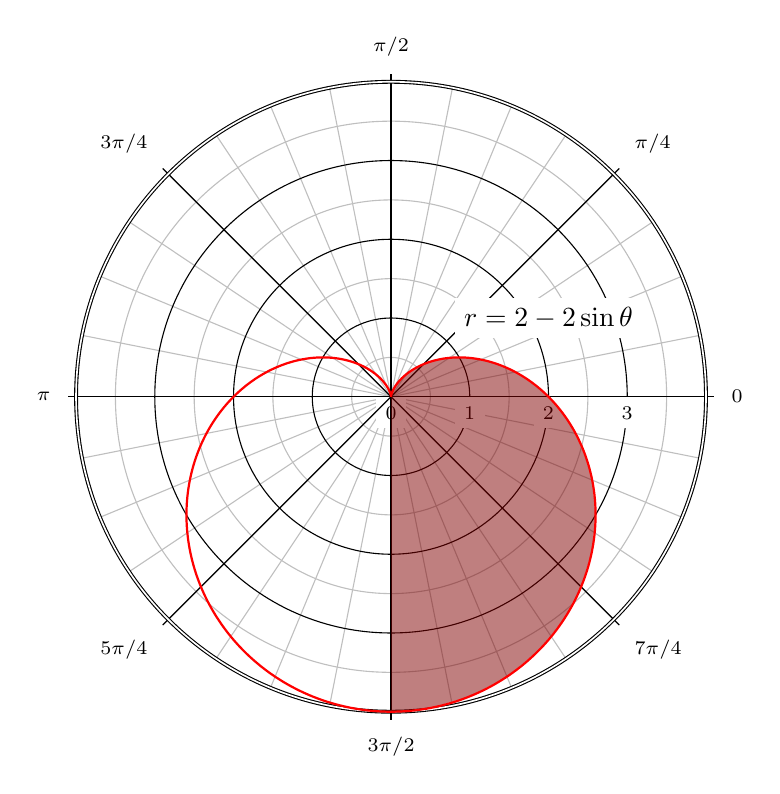
\begin{tikzpicture}[>=latex]
		% Draw the lines at multiples of pi/12
		\foreach \ang in {0,...,31} {
			\draw [lightgray] (0,0) -- (\ang * 180 / 16:4);
		}
		
		% Concentric circles and radius labels
		\foreach \s in {0, 1, 2, 3} {
			\draw [lightgray] (0,0) circle (\s + 0.5);
			\draw (0,0) circle (\s);
			\node [fill=white] at (\s, 0) [below] {\scriptsize $\s$};
		}
		
		% Add the labels at multiples of pi/4
		\foreach \ang/\lab/\dir in {
			0/0/right,
			1/{\pi/4}/{above right},
			2/{\pi/2}/above,
			3/{3\pi/4}/{above left},
			4/{\pi}/left,
			5/{5\pi/4}/{below left},
			7/{7\pi/4}/{below right},
			6/{3\pi/2}/below} {
			\draw (0,0) -- (\ang * 180 / 4:4.1);
			\node [fill=white] at (\ang * 180 / 4:4.2) [\dir] {\scriptsize $\lab$};
		}
		
		% The double-lined circle around the whole diagram
		\draw [style=double] (0,0) circle (4);
		
		\fill [fill=red!50!black, opacity=0.5] plot [domain=-pi/2:pi/2]
			(xy polar cs:angle=\x r, radius= {2-2*sin(\x r)});
		\draw [thick, color=red, domain=0:2*pi, samples=200, smooth]
			plot (xy polar cs:angle=\x r, radius={2-2*sin(\x r)});
		\node [fill=white] at (2,1) {$r=2-2\sin\theta$};
	\end{tikzpicture}
\caption{My polar plot}
\label{tikz:MyPolarPlot}
\end{figure}



\begin{figure}[h]
\centering 
\includegraphics[height=1.5in]{./pics/trim}
\caption{Caption for my figure4}
\label{fig:MyFigure4}
\end{figure}

















%%%%%%%%%%%%%%%%%%%%%%%%%%%%%%%%%%%%%%%%%
%	Typesetting Algorithms
\input{./algor/algorithms}


%%%%%%%%%%%%%%%%%%%%%%%%%%%%%%%%%%%%%%%%%
%	Bibliography
%\input{./others/bibliography}




%%%%%%%%%%%%%%%%%%%%%%%%%%%%%%%%%%%%%%%%%%%%%
%%%%%%%%%%%%%%%%%%%%%%%%%%%%%%%%%%%%%%%%%%%%%
%
%	End of document
%
%	Inserting references
%
%%%%%%%%%%%%%%%%%%%%%%%%%%%%%%%%%%%%%%%%%%%%%
%%%%%%%%%%%%%%%%%%%%%%%%%%%%%%%%%%%%%%%%%%%%%
%	Beginning of BACK MATTER: bibliography, indexes and colophon
%\backmatter
\appendix

{\linespread{1}
\bibliographystyle{plain}
\bibliography{./references/references}
\addcontentsline{toc}{chapter}{Bibliography}
}
\end{document}